\documentclass[tikz,border=14pt]{standalone}
\usepackage{lmodern}\usepackage{amsmath}\usepackage{amssymb}\usepackage{tikz}\usepackage{pgfplots}\pgfplotsset{compat=1.17}
\usetikzlibrary{calc,arrows.meta,positioning,patterns,decorations.markings,angles,quotes}
\definecolor{NebulaNavy}{HTML}{0B1F3A}
\definecolor{NebulaError}{HTML}{7952A3}
\definecolor{NebulaCheck}{HTML}{2E7D5B}
\definecolor{NebulaAmber}{HTML}{B47916}
\definecolor{NebulaGold}{HTML}{B77916}
\definecolor{NebulaLight}{HTML}{E4EAF0}
\definecolor{NebulaMuted}{HTML}{6E7E90}
\definecolor{NebulaNavyTwo}{HTML}{0B1F3A}
\definecolor{NebulaBG}{HTML}{F6F8FB}
\definecolor{NebulaSoft}{HTML}{E4EAF0}
\tikzset{
 nbline/.style={NebulaNavy,thick},
 nbdash/.style={NebulaNavy,thick,dashed},
 nbmass/.style={NebulaNavy},
 nbvec/.style={NebulaError,very thick,-{Stealth[length=2mm]}},
 nbvecb/.style={NebulaCheck,very thick,-{Stealth[length=2mm]}},
 nbaxis/.style={NebulaNavy,thick,-{Stealth[length=2mm]}},
}
\tikzset{nblabel/.style={NebulaNavy}}
\newcommand{\nbfuncplotlab}[9]{%
\pgfmathsetmacro{\nbyzero}{(0-(#3))/((#4)-(#3))}%
\begin{tikzpicture}
\begin{axis}[
  width=11.5cm, height=7.0cm,
  axis lines=middle,
  axis line style={NebulaNavy,-{Stealth[length=2mm]}},
  xmin=#1, xmax=#2, ymin=#3, ymax=#4,
  xlabel={#7}, ylabel={#8},
  xlabel style={at={(axis description cs:1.0,\nbyzero)},anchor=west,font=\small},
  ylabel style={at={(axis description cs:0.0,1.0)},anchor=south,font=\small},
  xtick distance=#5, ytick distance=#6,
  xticklabel style={font=\footnotesize,anchor=north,fill=white,inner sep=1.6pt},
  yticklabel style={font=\footnotesize,anchor=east,fill=white,inner sep=1.6pt},
  grid=both, grid style={NebulaMuted!45,very thin},
  tick style={NebulaNavy},
  clip=false
]
#9
\end{axis}
\end{tikzpicture}%
}
\begin{document}
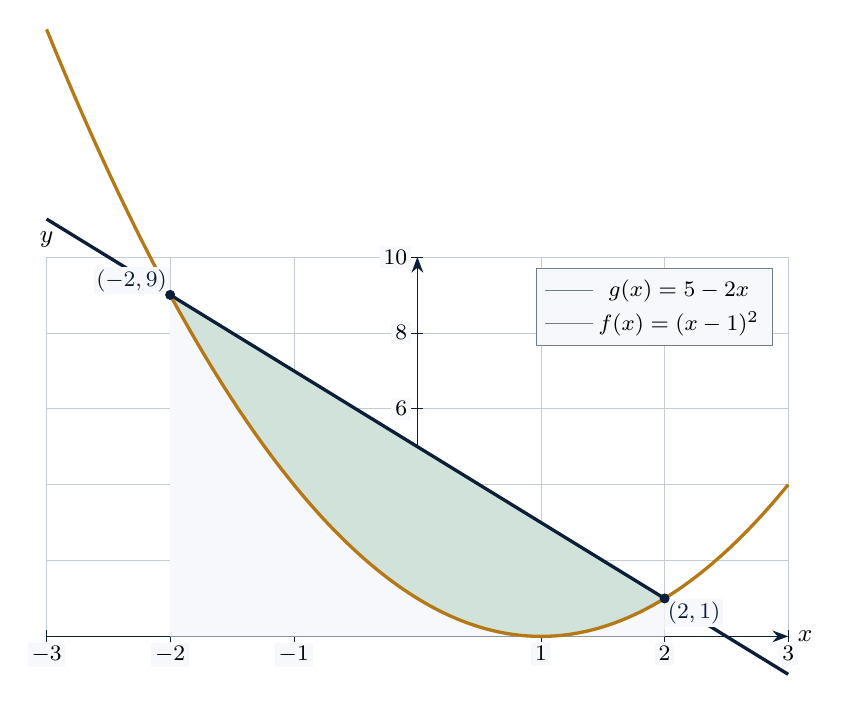
\begin{tikzpicture}
\begin{axis}[
  width=11.0cm, height=6.4cm, axis lines=middle,
  axis line style={NebulaNavy,-{Stealth[length=2mm]}},
  xmin=-3, xmax=3, ymin=0, ymax=10,
  xlabel={$x$}, ylabel={$y$},
  xlabel style={at={(axis description cs:1.0,0.000)},anchor=west,font=\small},
  ylabel style={at={(axis description cs:0.0,1.0)},anchor=south,font=\small},
  xtick distance=1, ytick distance=2,
  xticklabel style={font=\footnotesize,anchor=north,fill=NebulaBG,inner sep=1.4pt},
  yticklabel style={font=\footnotesize,anchor=east,fill=NebulaBG,inner sep=1.4pt},
  grid=both, grid style={NebulaMuted!40,very thin}, tick style={NebulaNavy}, clip=false,
  legend style={font=\footnotesize,draw=NebulaMuted,fill=NebulaBG,at={(0.98,0.97)},anchor=north east},
]
\addplot[draw=none,fill=NebulaCheck!22,domain=-2:2,samples=200] {5-2*x} \closedcycle;
\addplot[draw=none,fill=NebulaBG,domain=-2:2,samples=200] {(x-1)^2} \closedcycle;
\addplot[NebulaNavy,very thick,smooth,samples=200,domain=-3:3] {5-2*x};
\addplot[NebulaAmber,very thick,smooth,samples=200,domain=-3:3] {(x-1)^2};
\addplot[only marks,mark=*,NebulaNavy,mark size=1.6pt] coordinates {(-2,9)};
\node[font=\footnotesize,NebulaNavy,anchor=south east,fill=NebulaBG,inner sep=1pt] at (axis cs:-2,9) {$(-2,9)$};
\addplot[only marks,mark=*,NebulaNavy,mark size=1.6pt] coordinates {(2,1)};
\node[font=\footnotesize,NebulaNavy,anchor=north west,fill=NebulaBG,inner sep=1pt] at (axis cs:2,1) {$(2,1)$};
\legend{$g(x)=5-2x$,$f(x)=(x-1)^2$}
\end{axis}
\end{tikzpicture}
\end{document}
